\documentclass[11pt, a4paper]{article}

\usepackage{style}

\author{Vladislav Mlejnecký}

\title{%
  Číslicové zpracování signálů\\
  \large Úloha číslo 10.\\
  Aplikace filtrů - detektor tónové volby - simulace pomocí Matlab}

\begin{document}

    \maketitle

    \section{Zadání}
    
        Známým postupem nejprve vygenerujeme v Matlabu simulační signál představující posloupnost krátkých
        intervalů, ve kterých bude obsažena dvojice tónů odpovídající kódu DTMF. Na tuto část bude navazovat část
        detekční, která ze simulačního signálu rozpozná odpovídající číslice. Detekce bude spočívat ve vyhledávání
        současného výskytu tonů. Tóny budeme rozpoznávat jako nadprahový signál na výstupu příslušného filtru
        z banky filtrů. Banka filtrů bude obsahovat filtry pro všechny tóny kódu. Pro zjedodušení budeme filtrovat
        nikoliv současně, ale postupně po jednom kmitočtu, jde o off-line zpracování.
        
        \begin{enumerate}
     
            \item
            Vygenerujte signál tónové volby DTMF (Dual-tone multi-frequency) 
            postupně pro všechny číslice 0 až 9, * ,\# do jednoho souboru 
            (proměnné). Zvolte vzorkovací kmitočet 8000Hz, délka signálu pro jednu 
            číslici je 400 vzorků

            \item
            Navrhněte a pomocí funkcí Matlabu realizujte filtry pro jednotlivé 
            kmitočty. Filtry postupně aplikujte na složený tónový signál a každý 
            filtrovaný průběh zobrazte – viz vedlejší obrázek. Vyzkoušejte různé 
            aproximace a stupně filtrů a vyberte nejvhodnější.

            \item
            Vhodnými operacemi (abs. hodnota a práh) zpětně detekujte stisknuté 
            klávesy a výsledek zobrazte graficky tak, že do jednoho okna grafu 
            vložíte časové průběhy, které budou ukazovat hodnotou 1, že příslušná 
            klávesa byla stisknuta a hodnotou 0 nestisknutí – viz obrázek úplně 
            vpravo.
        
            \item            
            Nakreslete spektrogram složeného signálu a jednoho 
            vybraného filtrovaného signálu, např. 770 Hz.
        
        \end{enumerate}
    
        \begin{table}[H]
            \centering
            \begin{tabular}{|l|l|l|l|}
                \hline
                F [Hz] & 1209 & 1336 & 1477 \\ \hline
                697 & 1 & 2 & 3 \\ \hline
                770 & 4 & 5 & 6 \\ \hline
                852 & 7 & 8 & 9 \\ \hline
                941 & * & 0 & \# \\ \hline
            \end{tabular}
            \caption{Kmitočty tónové volby}
            \label{tab:1}
        \end{table}
    
    \section{Výsledné grafy}
            
        \begin{figure}[H]
            \centering
            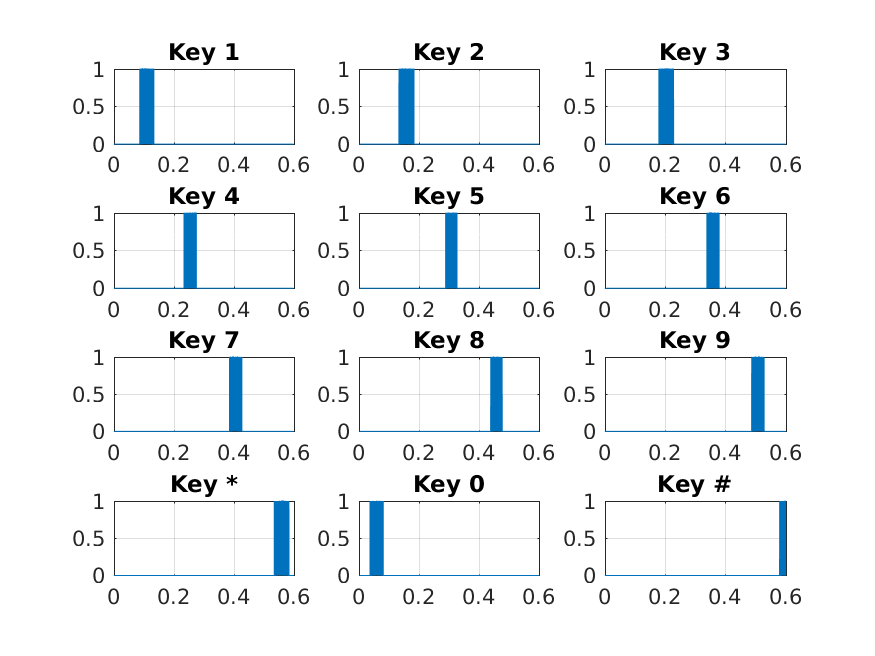
\includegraphics[width=.7\textwidth]{matlab/pressed.png}
            \caption{Vyfiltrované stisky kláves}
            \label{fig:1}
        \end{figure}
        
        \begin{figure}[H]
            \centering
            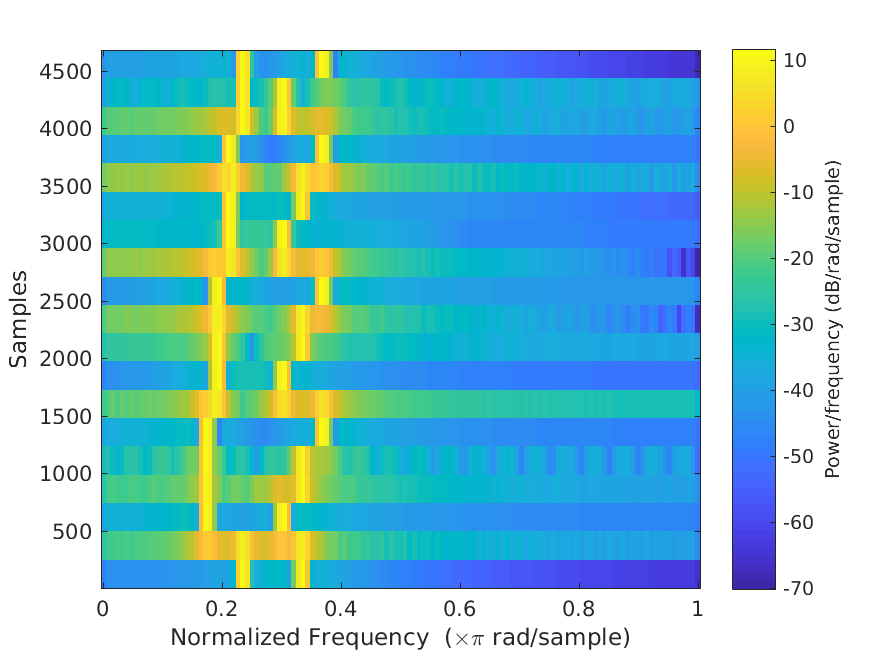
\includegraphics[width=.7\textwidth]{matlab/specgram_vector.png}
            \caption{Spektrum signálu s DTMF}
            \label{fig:2}
        \end{figure}
    
    \section{Výpis zdrojového kódu}
    
\begin{lstlisting}[language=matlab, frame=single] 
Fs = 8000;
n = 400;

y = make_vector('0123456789*#', Fs, n);
results = filter_keys(y, Fs);
make_key_graph(results, Fs, 'pressed');
make_specgram(y, 'specgram_vector');

function make_specgram(vector, FileName)
    h = figure();
    spectrogram(vector, 256, 10, 256);
    saveas(h, [FileName '.png']);
    close(h);
    clear h;
end

function make_key_graph(x, Fs, FileName)
    keyname = ['1', '2', '3', '4', '5', '6',...
               '7', '8', '9', '*', '0', '#'];
    
    t = (0:length(x) -1)/Fs;
    
    h = figure();
    for i = 1:12
        subplot(4, 3, i);
        plot(t, x(i,:));
        
        hold on;
        grid on; 
        
        xlim([0 length(x)/Fs]);
        ax = gca;
        ax.XTick = linspace(0, length(x)/Fs, 4);
        
        title(['Key ' keyname(i)]); 
    end
    saveas(h, [FileName '.png']);
    close(h);
end

function y = filter_keys(x, Fs)
    
    Ftones = [697, 770, 852, 941, 1209, 1336, 1477];
    
    d = 20;
    n = 6;
    a = zeros(7, 2*n+1);
    b = zeros(7, 2*n+1);
    
    for i = 1:7
        Ws = (2/Fs) .* [Ftones(i)-d Ftones(i)+d];
        [b(i,:), a(i,:)] = butter(n, Ws, 'bandpass');
    end
    
    y = zeros(12, length(x));
    
    y(1,:)  = filter(b(1,:), a(1,:), x) .* filter(b(5,:), a(5,:), x);
    y(2,:)  = filter(b(1,:), a(1,:), x) .* filter(b(6,:), a(6,:), x);
    y(3,:)  = filter(b(1,:), a(1,:), x) .* filter(b(7,:), a(7,:), x);

    y(4,:)  = filter(b(2,:), a(2,:), x) .* filter(b(5,:), a(5,:), x);
    y(5,:)  = filter(b(2,:), a(2,:), x) .* filter(b(6,:), a(6,:), x);
    y(6,:)  = filter(b(2,:), a(2,:), x) .* filter(b(7,:), a(7,:), x);

    y(7,:)  = filter(b(3,:), a(3,:), x) .* filter(b(5,:), a(5,:), x);
    y(8,:)  = filter(b(3,:), a(3,:), x) .* filter(b(6,:), a(6,:), x);
    y(9,:)  = filter(b(3,:), a(3,:), x) .* filter(b(7,:), a(7,:), x);

    y(10,:) = filter(b(4,:), a(4,:), x) .* filter(b(5,:), a(5,:), x);
    y(11,:) = filter(b(4,:), a(4,:), x) .* filter(b(6,:), a(6,:), x);
    y(12,:) = filter(b(4,:), a(4,:), x) .* filter(b(7,:), a(7,:), x);
    
    for i = 1:12
        y(i,:) = y(i,:) .* y(i,:) > 0.1;
    end
    
end

function y = make_vector(keys, Fs, n)
    vector = zeros(1, n * length(keys));
    
    for i = 1:length(keys)
        vector( i*n-n+1 : i*n ) = dtfm(keys(i), Fs, n);
    end
    
    y = vector;
end
        
function y = dtfm(key, Fs, n)
    t = (0:n-1)/Fs;
    
    switch key
        case '0'
            f1 = 941; f2 = 1336;
        case '1'
            f1 = 697; f2 = 1209;
        case '2'
            f1 = 697; f2 = 1336;
        case '3'
            f1 = 697; f2 = 1477;
        case '4'
            f1 = 770; f2 = 1209;
        case '5'
            f1 = 770; f2 = 1336;
        case '6'
            f1 = 770; f2 = 1477;
        case '7'
            f1 = 852; f2 = 1209;
        case '8'
            f1 = 852; f2 = 1336;
        case '9'
            f1 = 852; f2 = 1477;
        case '*'
            f1 = 941; f2 = 1209;
        case '#'
            f1 = 941; f2 = 1477;
        otherwise
            f1 = 0; f2 = 0;
    end
    
    w1 = 2 * pi * f1;
    w2 = 2 * pi * f2;
    
    y = sin(w1 * t) + sin(w2 * t);
    
end
\end{lstlisting}        

\end{document}
